\section{Versuchsdurchführung und Auswertung}
	\subsection{Einstellen der Betriebsparameter}
		Um die folgenden Messungen unter möglichst günstigen Bedingungen durchführen zu können, wurden zunächst unter Anweisung des Betreuers die Betriebsparameter der Ionenfalle überprüfung und gegebenenfalls optimiert:
		\begin{itemize}
			\item linke Potentialwand $U_0 = \unit[11,857]{kV}$
			\item Potentialtopf ($\hat{=}$ Beschleunigungsspannung) $U_A = \unit[11,707]{kV}=U_B$
			\item rechte Potentialwand $U_{B1} = \unit[12,007]{kV}$
			\item Extraktionszeit $t_{ext} = \unit[20]{ms}$
		\end{itemize}
		Da die Abhängigkeit der Argonionisationen von Arbeitsdruck und Ionisationszeit innerhalb des Strahlrohrs untersucht werden soll, werden diese in den folgenden Abschnitten genauer spezifiziert. Abbildung \ref{fig:potentialkasten} skizziert nochmals die Potentialverhältnisse entlang der Strahlachse.
		\begin{figure}[htb]
			\centering
			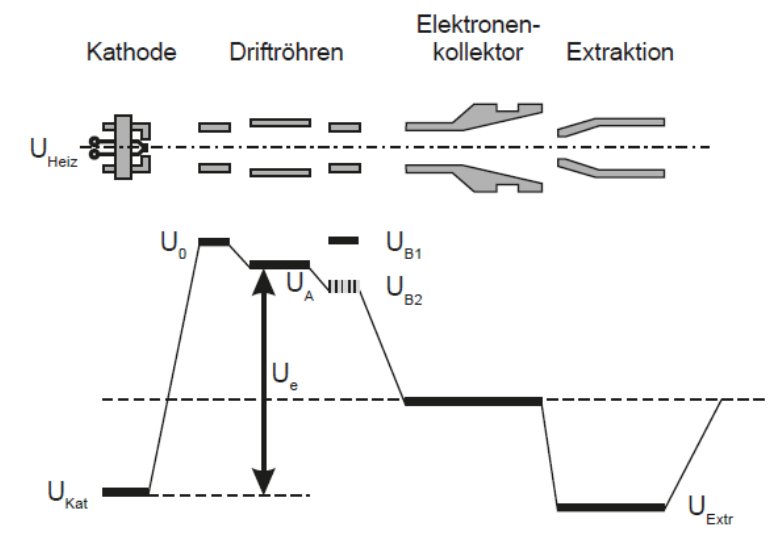
\includegraphics[width=0.8\linewidth]{pic/potentialkasten}
			\caption{Elektrodenanordnung (oben) mit zugehörigem Potentialverlauf in der Ionenfalle.\cite{PA}}
			\label{fig:potentialkasten}
		\end{figure}
		
	\subsection{Aufnahme und Analyse eines Übersichtsspektrums}
		Um die einzelnen Ionisationszustände des Argons sauber voneinander trennen zu können, ist es notwendig zu wissen, wie man den Strom des 90°-Dipol-Magneten wählen muss. Im Experiment sollen die Ionen Ar$^{8+}$ bis Ar$^{18+}$ untersucht werden. Mit Hilfe von Formel (\ref{eq:radius}) wird das Magnetfeld abgeschätzt, um die gewünschten Ionen auszufiltern. Es ergibt sich ein Messintervall von $B = 50,4 \dots \unit[75,6]{mT}$, wobei die untere Grenze den höchsten Ionisationszustand Ar$^{18+}$ und die untere Grenze den niedrigsten Zustand Ar$^{8+}$ herausfiltert. Die Einstellung dieser Magnetflussdichten erfolgt über die Variation des Spulenstroms von $\unit[17,3]{A}$ bis $\unit[27,2]{A}$. 
		Bei der ersten Messung wurde die Ionisationszeit mit $t_{ion} = \unit[380]{ms}$ zu hoch gewählt, um damit niedrigere Ladungszustände als Ar$^{13+}$ zu erzeugen. Dieser Effekt wird im zweiten Versuchsteil näher erörtert. Abbildung \ref{fig:7e-9} zeigt das dabei entstandene Übersichtsspektrum, welches bei mittlerem Arbeitsdruck von $p = \unit[7\cdot 10^{-9}]{mbar}$ entstanden ist. Die Ladung $Q$ wurde dabei über 5 Zyklen integriert.		
		Um ein vollständiges Übersichtsspektrum zu erhalten, wurde die Messung am Ende des Versuchstages mit einer niedrigeren Ionisationszeit $t_{ion} = \unit[80]{ms}$ und einem nicht signifikant erhöhten Arbeitsdruck $p = \unit[2\cdot 10^{-8}]{mbar}$ wiederholt. Diese Wahl maximiert die Häufigkeit von mittleren Ionisationszuständen um Ar$^{12}$ und ermöglicht die Messung aller möglicher Peaks. Abbildung \ref{fig:2e-8} zeigt das zugehörige Übersichtsspektrum, bei dem ebenfalls über 5 Zyklen integriert wurde.\\
		\begin{figure}[h]
		    \centering
		    \begin{minipage}{0.9\linewidth}
		        \centering
		        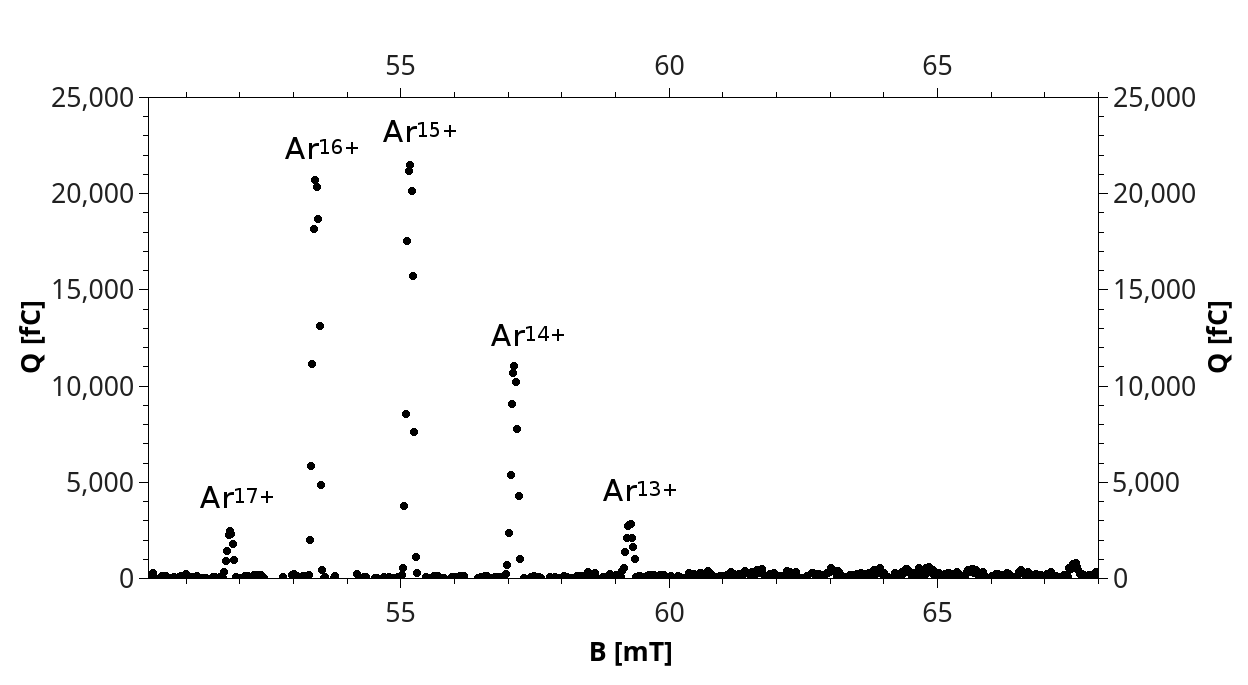
\includegraphics[width=0.8\linewidth]{pic/7e-9_beschriftet}
		        \caption{Übersichtsspektrum bei $p = \unit[7\cdot 10^{-9}]{mbar}$ und $t_{ion} = \unit[380]{ms}$. Die Peaks niedriger Ladungszustände verschwinden aufgrund der zu hohen Ionisationszeit.}
		        \label{fig:7e-9}
		    \end{minipage}
		    \vfill
		    \begin{minipage}{0.9\linewidth}
		        \centering
		        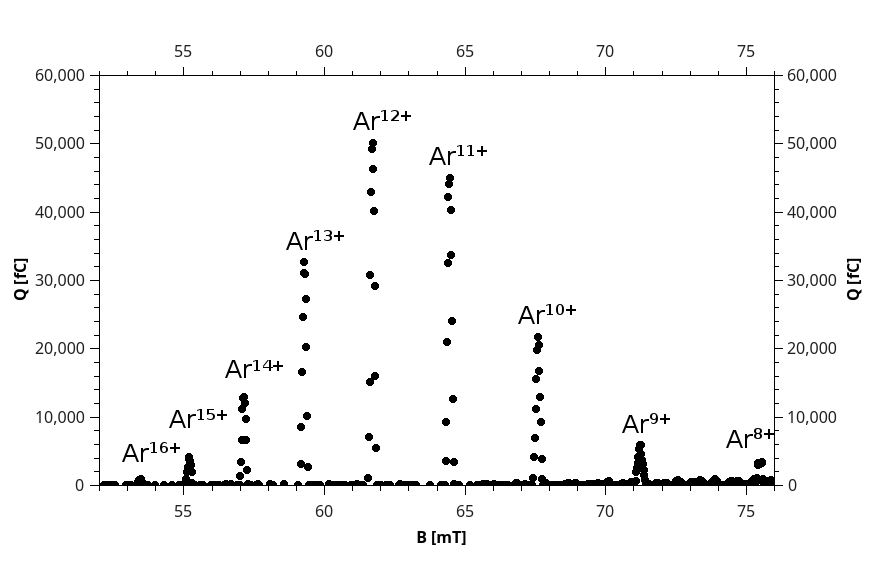
\includegraphics[width=0.8\linewidth]{pic/2e-8_beschriftet}
		        \caption{Übersichtsspektrum bei mittlerem Arbeitsdruck $p = \unit[2\cdot10^{-8}]{mbar}$ und $t_{ion} = \unit[80]{ms}$. Alle gewünschten Peaks sind erkennbar, da nun mittlere Ladungszustände am häufigsten auftreten.}
		        \label{fig:2e-8}
		    \end{minipage}
		\end{figure}
		\ \\
		Durch Ermitteln der Peakpositionen erhält man die Magnetflussdichten, die im zweiten Versuchsteil genutzt werden sollen, um die Ladungszustände zu isolieren. Um zu prüfen, ob die in Abbildung \ref{fig:2e-8} eingezeichnete Zuordnung korrekt ist, wurde ein quadratischer Fit der reziproken relativen Ladung $e/Q$, welche nach (\ref{eq:Q}) proportional zu $B^2$ ist, vorgenommen.
		\begin{equation} \label{eq:Q}
		\frac{1}{q} = \frac{e}{Q} = \frac{r^2 e}{2 U_B m_{Ar}}\cdot B^2 \simeq \unit[21,92]{\frac{1}{T^2}} \cdot B^2
		\end{equation} 
		Wobei $m_{Ar} = \unit[39,9]{u}$ die Masse von Argon ist. Abbildung \ref{fig:quadr_fit} zeigt das Ergebnis dieses Fits mit dem Ansatz $1/q = A\cdot B^2$. Dabei wurde die Proportionalitätskonstante mit $A = (21,7 \pm 0,1)\unit{/T^2}$ bestimmt, was nach (\ref{eq:Q}) sehr gut zum theoretischen Wert passt.\\
		%Einen weiteren Beleg für die gute Übereinstimmung der aufgenommenen Messwerte mit den aus (\ref{eq:radius}) theoretisch berechneten Werten zeigt Tabelle \ref{tab:data_fit}, welche beide direkt miteinander vergleicht.\\
		\begin{figure}[htb]
			\centering
			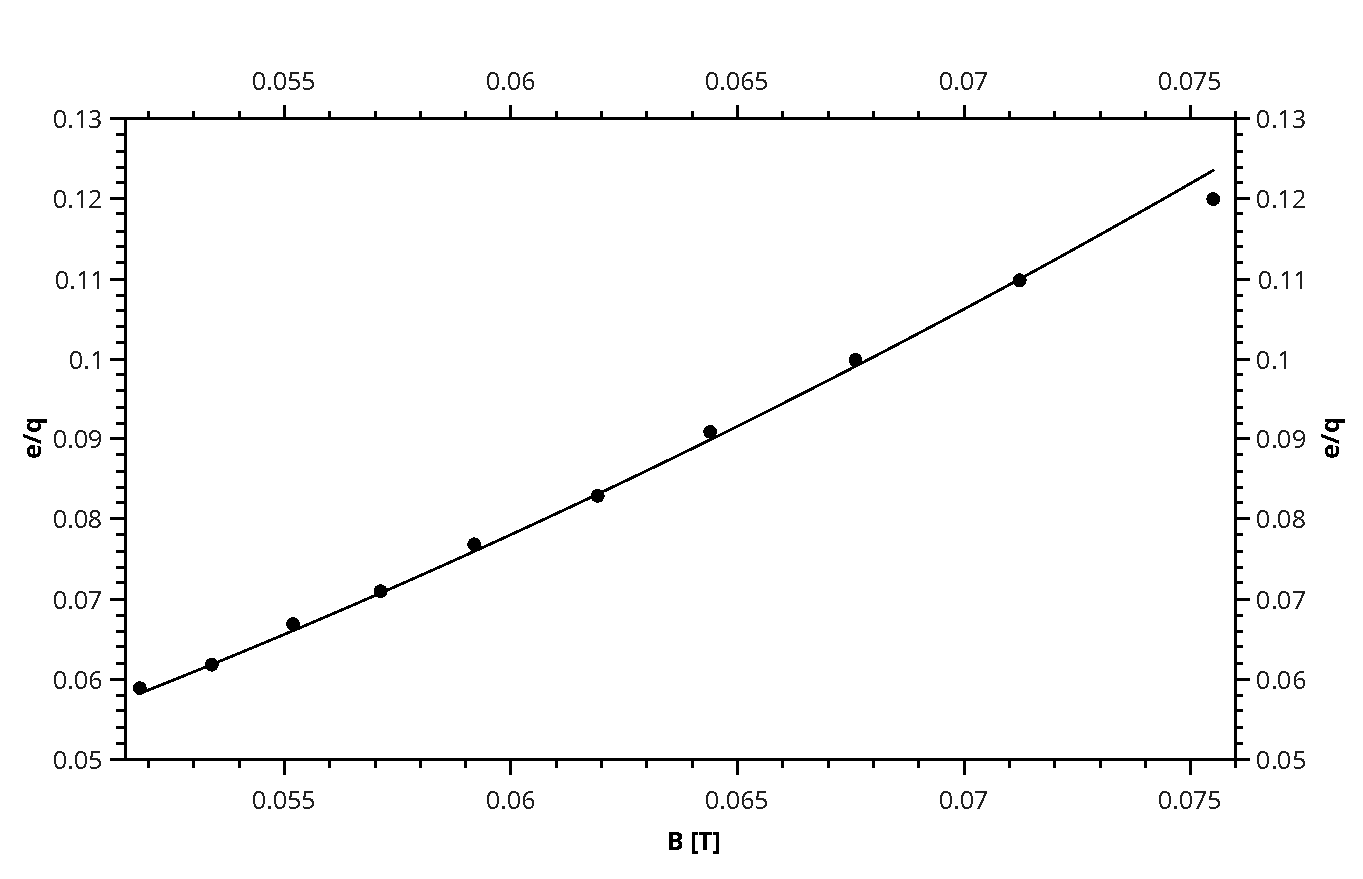
\includegraphics[width=\linewidth]{pic/quadr_fit.pdf}
			\caption{Quadratischer Fit, um Zuordnung der Peaks aus Abbildung \ref{fig:2e-8} zu verifizieren.}
			\label{fig:quadr_fit}	
		\end{figure}
		%\begin{table}[htb]
		%	\centering
		%	\begin{tabular}{c|c|c|c}
		%		$q = \frac{Q}{e}$ & $B_{experimentell}$ [mT] & $B_{theoretisch}$ [mT] & $1/q = e/Q$\\
		%		\hline 
		%		17	&	51,83	&	51,77	&	0,059\\
		%		16	&	53,39	&	53,36	&	0,062\\
		%		15	&	55,15	&	55,11	&	0,067\\
		%		14	&	57,09	&	57,05	&	0,071\\
		%		13	&	59,23	&	59,20	&	0,077\\
		%		12	&	61,67	&	61,62	&	0,083\\
		%		11	&	64,42	&	64,36	&	0,091\\
		%		10	&	67,52	&	67,50	&	0,100\\
		%		9	&	71,14	&	71,15	&	0,111\\
		%		8	&	75,52	&	75,47	&	0,12
		%	\end{tabular}
		%	\caption{Ermittelte Magnetflussdichten, die die gewünschten Ionisationszustände auf eine Kreisbahn mit korrektem Radius lenken.}
		%	\label{tab:data_fit}
		%\end{table}
	\subsection{Einfluss des Drucks auf die Ionenzustände im Strahlkanal}
		Um den Einfluss des Arbeitsdrucks im Niederenergiestrahlkanal zu untersuchen, wurden zwei weitere Übersichtsspektren mit gleicher Ionisationszeit von $t_{ion} = \unit[380]{ms}$ und Messzeit von $t_{mess} = \unit[2000]{ms}$ (5 Zyklen), aber mit verschiedenen Drücken aufgenommen. Abbildung \ref{fig:all} zeigt dabei den direkten Vergleich vom Spektrum mit niedrigem Arbeitsdruck $p_1 = \unit[2\cdot 10^{-9}]{mbar}$ (rot) und hohem Arbeitsdruck $p_2 = \unit[5\cdot 10^{-8}]{mbar}$ (blau).\\
		\begin{figure}[htb]
			\centering
			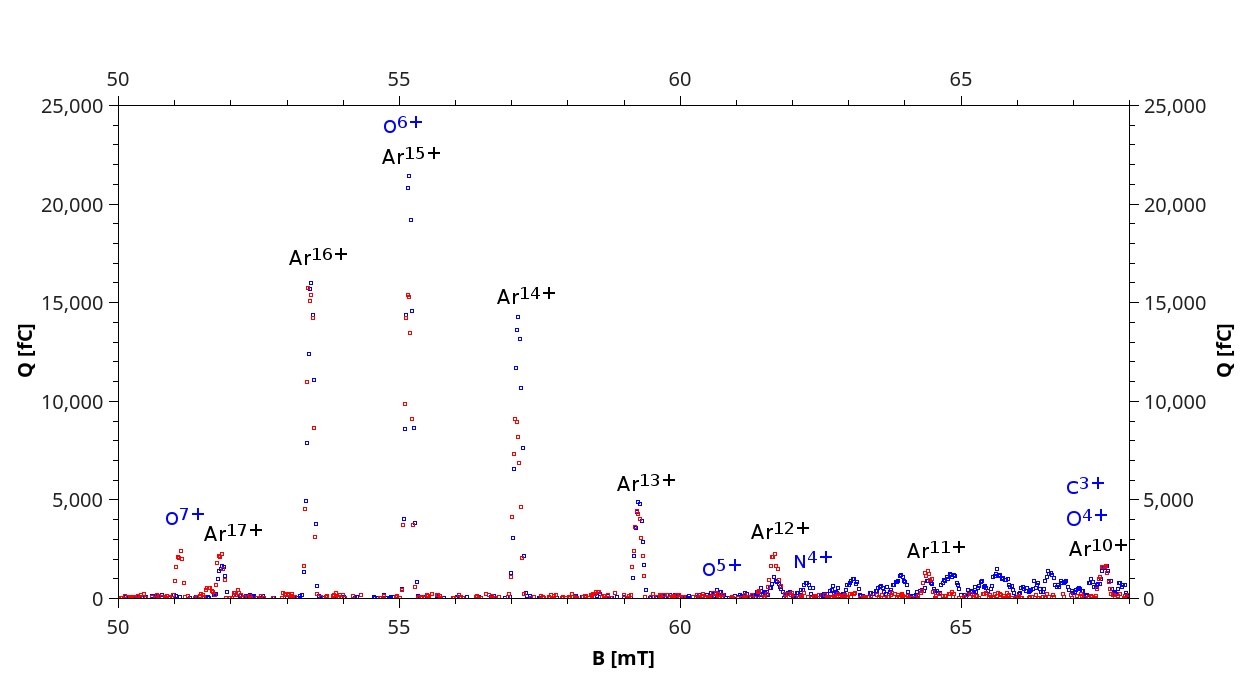
\includegraphics[width=\linewidth]{pic/all_beschriftet.png}
			\caption{Übersichtsspektrum mit $t_ion = \unit[380]{ms}$ unter verschiedenen Drücken $p_1 = \unit[2\cdot 10^{-9}]{mbar}$ (rot) und $p_2 = \unit[5\cdot 10^{-8}]{mbar}$ (blau). In blau beschriftete Peaks kennzeichnen mögliche Fremdionen im Strahlkanal.}
			\label{fig:all}	
		\end{figure}
		\ \\
		Es fällt auf, dass bei \textbf{niedrigen Drücken} ein viel geringerer Ionenstrom durch die Anlage fließt und somit am Faradaycup weniger Ladung pro Zeiteinheit nachgewiesen wird. Die kinetische Gastheorie liefert einen Zugang, um dies zu verstehen: Druck ist ein Maß für die Kraft, die Gasmoleküle auf die Gefäßwand ausüben. Je niedriger der Druck, desto weniger Kollisionen der Teilchen gibt es mit der Gefäßwand und auch untereinander. Dies führt zu einer geringeren mittleren Geschwindigkeit der Gasteilchen und somit zu einer geringeren Stromdichte $j = n\cdot Q \cdot v$, welche am Faradaycup als Ladung pro Zeiteinheit und Fläche nachgewiesen wird. Doch warum tritt diese Absenkung hauptsächlich bei mittleren Ionenzuständen (Ar$^{13+}$ bis Ar$^{15+}$) auf? Dies kann über die Verringerung des \textit{Ladungsaustauschs} zwischen den Ionen, der in Abschnitt \ref{sec:ww} näher erläutert wird, begründet werden. Die Häufigkeit dieses Prozesses sinkt bei niedrigem Druck, wodurch hochgeladene Ionen begünstigt werden und die Absenkung des Ionenstroms kompensiert wird.\\
		In Abbildung \ref{fig:all} ist bei etwa $\unit[51]{mT}$ ein roter Peak deutlich zu sehen. Diesen könnte man naiverweise aufgrund des niedrigen Drucks dem höchst angeregten Argonzustand Ar$^{18+}$ zuordnen. Das ist allerdings nicht der Fall, da die Theorie diesen bei etwa $\unit[50,4]{mT}$ erwarten würde. Man kann spekulieren, ob der Peak zu einem höchst angeregten Fremdion aus dem Strahlkanal gehört. Ein Atom, bei dem diese Zuordnung hervorragend funktioniert, ist Sauerstoff mit einer Masse von $m_O = \unit[16]{u}$. Der Peak zu O$^{7+}$ ist genau an der erwarteten Position und auch sonstige Maxima des Sauerstoffs passen sehr gut in das gemessene Spektrum herein, fallen aber teilweise mit denen des Argons zusammen.\\
		Bei \textbf{hohem Druck} ist nicht nur die mittlere Geschwindigkeit, sondern auch die Teilchenzahl und somit auch die Zahl an Fremdatomen im Strahlkanal deutlich höher. Da der Ladungsaustausch nun begünstigt wird und zudem der Ionenstrom größer ist, treten Peaks von gering angeregten Fremdionen als starkes Untergrundrauschen vor allem im Bereich hoher Magnetfelder auf. Das führt dazu, dass mittlere und niedrige Argonionisationszustände, die durch die hohe Ionisationszeit ohnehin unterdrückt sind, nicht mehr sauber herausgeefiltert werden können. In Abbildung \ref{fig:all} wurde ein Versuch unternommen, mögliche Fremdionen mit Saustoff-, Stickstoff- und Kohlenstoffatomen zu identifizieren. Dies ist allerdings rein spekulativ, da die Peaks nur sehr klein sind und man zu noch höheren Magnetfeldern hätte übergehen müssen. Außerdem fallen viele Maxima aufgrund gleicher spezifischer Ladung $Q/m$ zusammen, wodurch keine eindeutige Zuordnung möglich ist.\\
		Da die Anzahl der Ionen proportional zur am Faradaycup gemessenen Ladung ist, erhält man durch Verhältnisbildung eine grobe Abschätzung der Anzahl an Fremdatomen. Dafür sucht man Peaks, die mit keinem anderen Fremdatom zusammenfallen und die nach Möglichkeit dem am häufigsten auftretenden Ionenzustand entsprechen, z.B. von O$^{7+}$ und Ar$^{16+}$.
		\begin{equation}
			\frac{N_{O}}{N_{Ar}} = \frac{Q(\text{O}^{7+})}{Q(\text{Ar}^{16+})}\approx \unit[15,4]{\%}
		\end{equation}
		Das heißt, es befindet sich tatsächlich noch ein signifikanter Anteil an Fremdatomen im Strahlkanal, der mit den untersuchten Ionen wechselwirkt.
		
		%TODO@Christian: Zeitentwicklungen